\section{Extension to Nonlinear Plants}
\label{sec:nonlinear}

\subsection{Motivation}
\label{sec:nonlinear:motivation}

The KZV derivation in \cref{sec:methodology} assumes that the plant is
well-approximated by a linear FOPDT model~\eqref{eq:fopdt}.
Many industrial processes, however, exhibit parameter variation with operating
point.
In a cooling circuit, for example, the heat-transfer coefficient — and hence
the process gain~$K$ — decreases at higher temperatures, while thermal
capacitance effects tend to increase the dominant time constant~$T$.
Such behaviour is captured by a \emph{nonlinear FOPDT-like} plant:

\begin{align}
    K_{\mathrm{eff}}(y) &= K_0 \bigl(1 + \alpha_K (y - y_{\mathrm{ref}})\bigr),
    \label{eq:K_nonlin} \\
    T_{\mathrm{eff}}(y) &= T_0 \bigl(1 + \alpha_T (y - y_{\mathrm{ref}})\bigr),
    \label{eq:T_nonlin}
\end{align}
with constant dead time~$L$ and sensitivity coefficients $\alpha_K < 0$,
$\alpha_T > 0$.
The dead time $L$ is assumed constant across operating points; in practice,
transport and sensor delays may vary mildly, which is left for future study.
Here $y_{\mathrm{ref}}$ is the nominal operating point at which the FOPDT
model is exact.

\subsection{Local Linearisation and the KZV}
\label{sec:nonlinear:local}

A key property of the Bang-Bang limit cycle is that it oscillates around a
single setpoint~$r$.
In the limit of small hysteresis $d$, the entire oscillation is confined to a
neighbourhood of $r$, where the nonlinear plant~\eqref{eq:K_nonlin}--\eqref{eq:T_nonlin}
is locally linear with

\begin{equation}
    K \approx K_{\mathrm{eff}}(r), \quad T \approx T_{\mathrm{eff}}(r).
    \label{eq:local_lin}
\end{equation}

The KZV therefore estimates the \emph{local linearisation} of the plant at the
current setpoint, without any explicit knowledge of the nonlinearity.
This is the fundamental mechanism that makes KZV robust to mild plant
nonlinearities.

\begin{remark}
    The approximation~\eqref{eq:local_lin} becomes exact as $d \to 0$.
    For practical hysteresis values ($d \ll A_u$), the error in $K$ and $T$ is
    of order $\alpha \cdot A_u$, which is negligible for typical industrial
    nonlinearities.
\end{remark}

\subsection{Simulation Study}
\label{sec:nonlinear:sim}

To evaluate the KZV on a nonlinear plant, we use the model
\eqref{eq:K_nonlin}--\eqref{eq:T_nonlin} with nominal parameters
$K_0 = \SI{0.5}{\degreeCelsius\per\percent}$,
$T_0 = \SI{120}{\second}$, $L = \SI{20}{\second}$,
$y_{\mathrm{ref}} = \SI{20}{\degreeCelsius}$,
and sensitivity coefficients $\alpha_K = \SI{-0.01}{\per\degreeCelsius}$,
$\alpha_T = \SI{0.005}{\per\degreeCelsius}$.
At $y = \SI{28}{\degreeCelsius}$, this gives
$K_{\mathrm{eff}} \approx \SI{0.46}{\degreeCelsius\per\percent}$ (8\% below
nominal) and $T_{\mathrm{eff}} \approx \SI{124}{\second}$ (3\% above nominal).

\Cref{fig:nonlinear_param} shows the true parameter curves
\eqref{eq:K_nonlin}--\eqref{eq:T_nonlin} alongside the KZV estimates
obtained by running a separate Bang-Bang experiment at each setpoint.
The KZV closely tracks the local linearisation across the full operating
range of \SIrange{15}{30}{\degreeCelsius}.

\begin{figure*}[t]
    \centering
    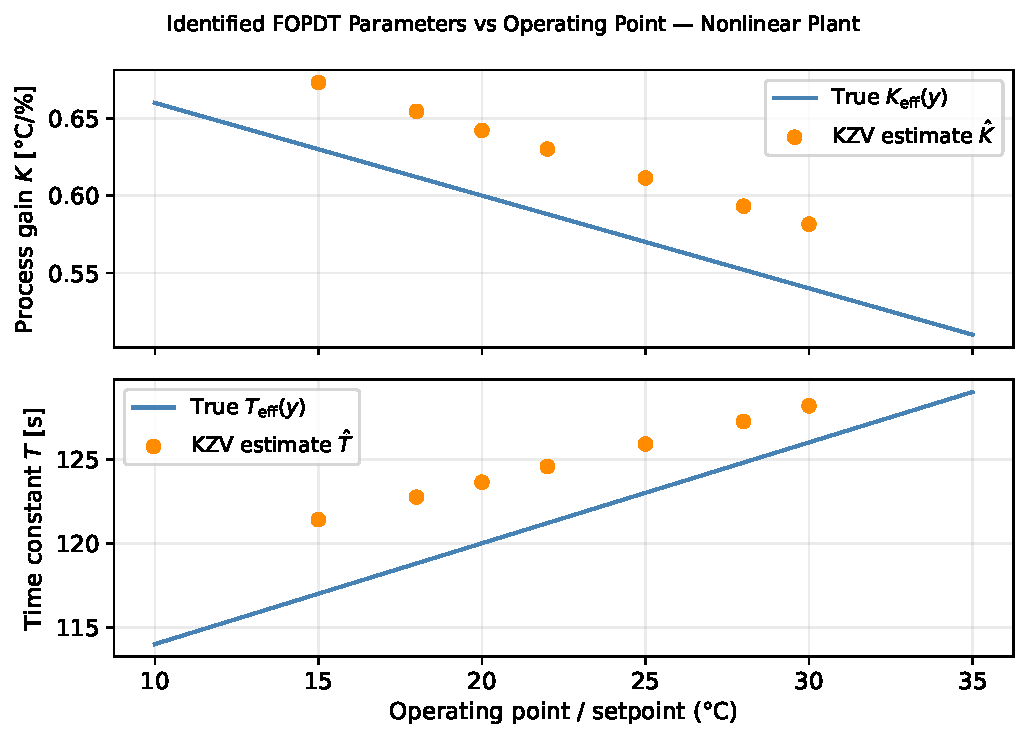
\includegraphics[width=0.92\linewidth]{figures/nonlinear_param_variation.pdf}
    \caption{True local FOPDT parameters $K_{\mathrm{eff}}(y)$ and
             $T_{\mathrm{eff}}(y)$ (solid lines) vs KZV estimates
             (markers) obtained from Bang-Bang experiments at each setpoint.
             Dead time $L$ is constant and is accurately recovered throughout
             (not shown).}
    \label{fig:nonlinear_param}
\end{figure*}

\subsection{Gain-Scheduled KZV}
\label{sec:nonlinear:gs}

The local-linearisation property suggests a simple gain-scheduling strategy:

\begin{enumerate}
    \item Run the KZV at $n$ representative operating points
          $\{r_1, r_2, \ldots, r_n\}$ spanning the expected range.
    \item Store the identified triples
          $(\hat{K}(r_i), \hat{T}(r_i), \hat{L}(r_i))$ as a look-up table.
    \item At runtime, interpolate the PID parameters
          $(\Kp, \Ti, \Td)$ as a function of the current setpoint~$r$.
\end{enumerate}

This is structurally equivalent to classical gain scheduling, but the
scheduling function is identified automatically from the plant's own
Bang-Bang limit cycles — no explicit plant model is required.

\Cref{fig:nonlinear_step} compares three PID configurations for a step to
$\SI{28}{\degreeCelsius}$:

\begin{enumerate}
    \item \textbf{Nominal KZV}: identified at $r = \SI{20}{\degreeCelsius}$
          and applied without adaptation.
    \item \textbf{Local KZV}: re-identified at $r = \SI{28}{\degreeCelsius}$
          (one-shot gain-scheduled).
    \item \textbf{Ideal local IMC}: tuned with the exact local parameters
          $K_{\mathrm{eff}}(28)$, $T_{\mathrm{eff}}(28)$ — serves as upper
          bound.
\end{enumerate}

\begin{figure*}[t]
    \centering
    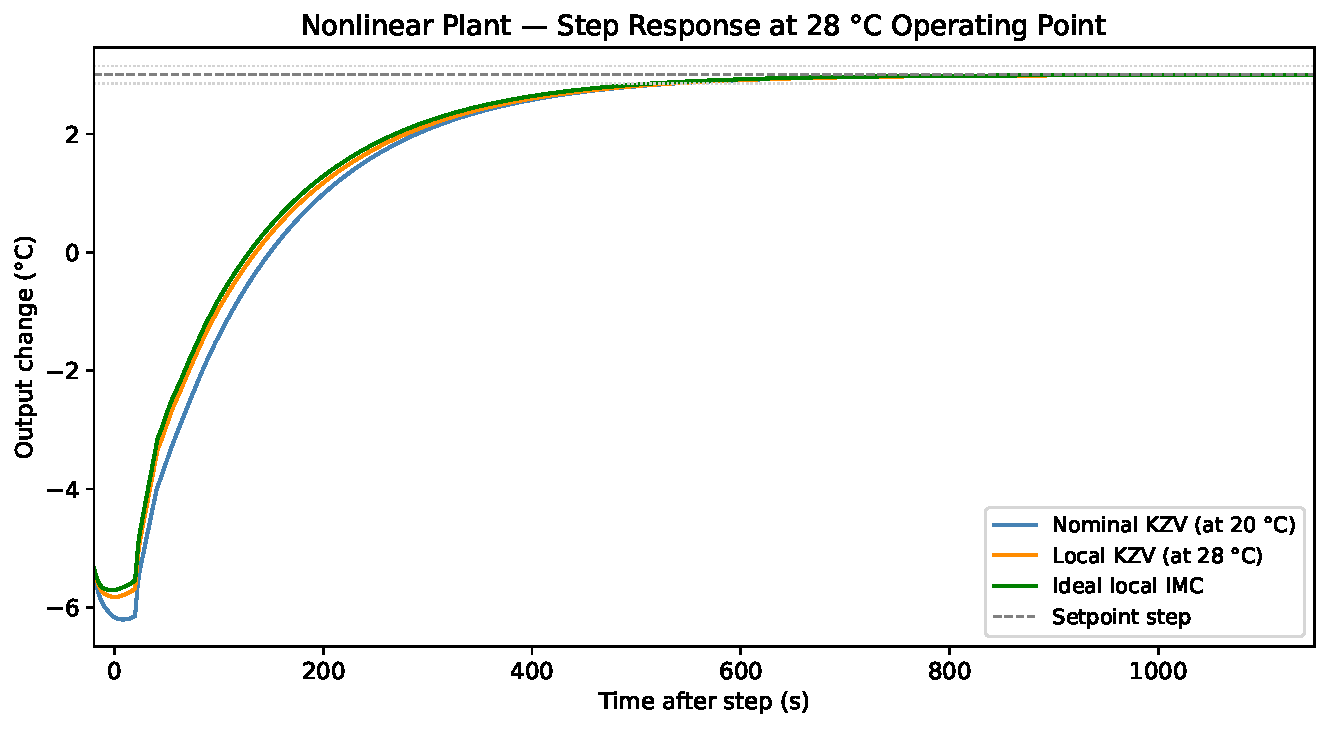
\includegraphics[width=0.92\linewidth]{figures/nonlinear_step_response.pdf}
    \caption{Closed-loop step responses on the nonlinear plant at the
             \SI{28}{\degreeCelsius} operating point.
             The locally re-identified KZV (orange) nearly matches ideal IMC
             performance, while the nominal KZV (blue, tuned at \SI{20}{\degreeCelsius})
             remains stable but exhibits a slower response.}
    \label{fig:nonlinear_step}
\end{figure*}

The nominal KZV remains stable at the off-nominal operating point, confirming
the inherent robustness of IMC tuning.
The local KZV achieves near-ideal performance, demonstrating that a
single additional Bang-Bang experiment at the new operating point is sufficient
to recover optimal performance.

\subsection{Validity Conditions}
\label{sec:nonlinear:validity}

The local linearisation assumption~\eqref{eq:local_lin} holds when:

\begin{itemize}
    \item The oscillation amplitude satisfies $A_u \ll 1/\alpha_{K,T}$,
          i.e.\ the parameter variation over one oscillation cycle is small.
    \item The nonlinearity is smooth (no discontinuities within the limit-cycle
          amplitude range).
    \item The dead time $L$ does not vary significantly with operating point.
\end{itemize}

Plants with strong nonlinearities (e.g.\ saturation, dead-band, or sharp
gain changes) may produce asymmetric limit cycles.
In such cases, the KZV estimates should be verified by inspecting the
symmetry of the oscillation: a ratio $T_{\text{on}} / T_{\text{off}}$
deviating from~1 by more than 10\% is a warning sign that the FOPDT
approximation is inadequate.
